\documentclass[
  report,
  a4paper,
  12pt,
  paperwidth=210mm,
  paperheight=297mm,
  hoffset=0mm,
  voffset=0mm,
  textwidth=175mm, % left=25mm, right=10mm
  textheight=267mm % top=15mm, bottom=15mm
]{jlreq}
\usepackage{array}
\usepackage{multirow}
\usepackage[dvipdfmx]{graphicx} % \resizebox用
\usepackage{subcaption} 

\begin{document}

\title{
スパイラルコア用リボンケーブルの

ダイリップ形状推定方法開発
}
\author{シセ-キ 小林}
\date{2025/08/28}
\maketitle

\chapter{概要}
スパイラルコア用リボン押出を対象とし、異形樹脂押出工程における CAE \footnote{Computer Aided Engineering}手法を検討した。

実製造工程と製品形状を数値化し、物理モデルと統計モデルで記述する方法、およびモデルの逆解析による製造工程最適化方法について説明する。

\chapter{背景}
スパイラルコア(\small{以下 "SC" と略})は、電力ケーブル接続部の絶縁処理部材 RBJ\footnote{Rubber Block Joint - 電力用ケーブル(主にCVケーブル)を接続する際に使われる、ゴムブロック絶縁型のジョイント(中間接続部材)} の装着時に使用される円筒状の部材である。この SC は SC 用リボンをらせん(\small{スパイラル})状に嵌合させ形成されており、嵌合時の強度と安定性を確保するために適切な断面形状が指定されている。

\begin{figure}
  \centering
    \begin{minipage}{0.4\columnwidth}
    \centering
    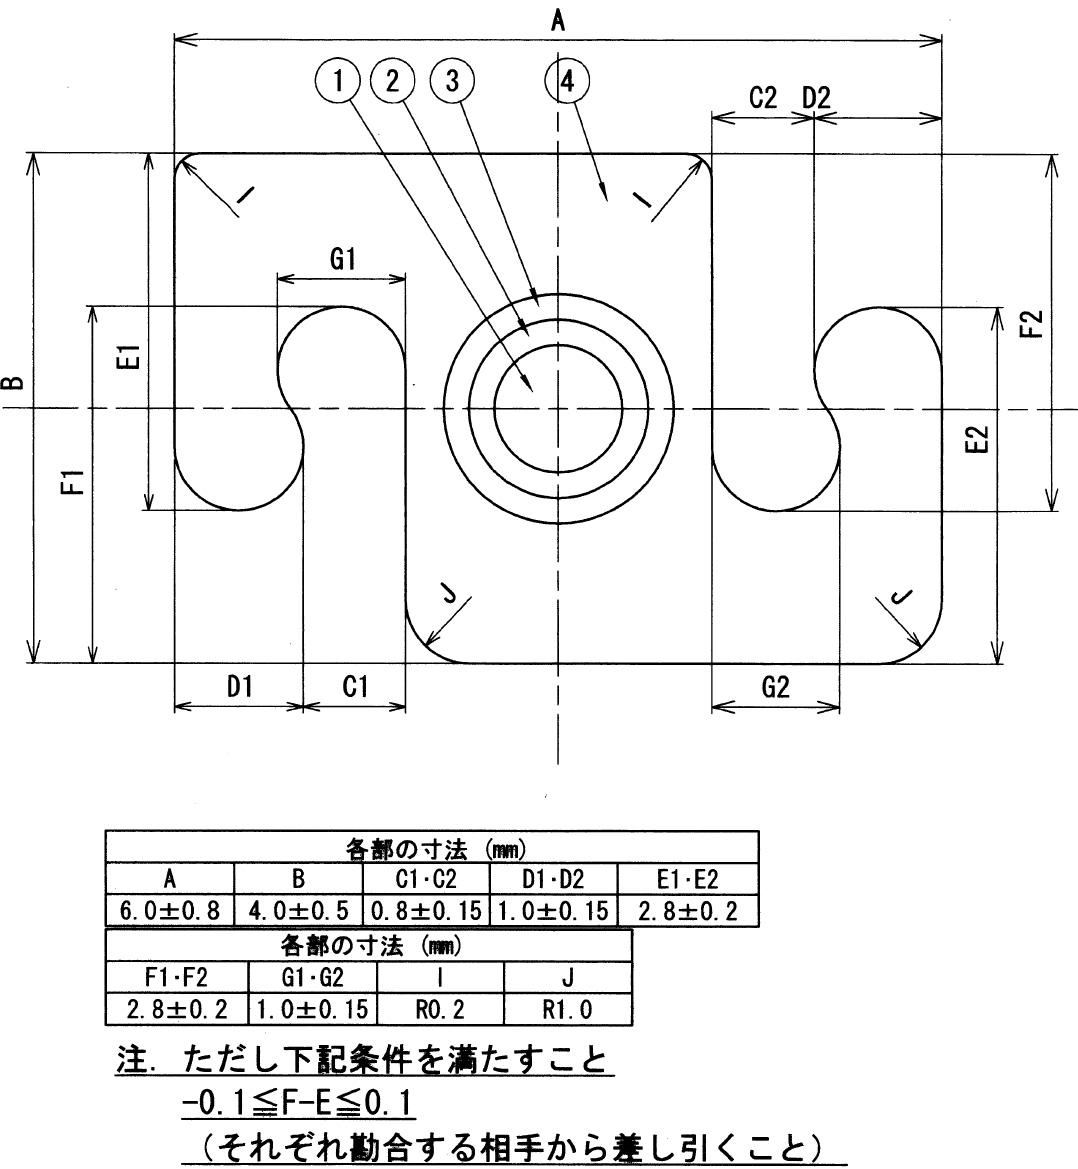
\includegraphics[width=\columnwidth]{SC_M-6-4.jpg}
    \caption{left}
    \label{fig:SC_M-6-4}
  \end{minipage}
  \begin{minipage}{0.4\columnwidth}
    \centering 
    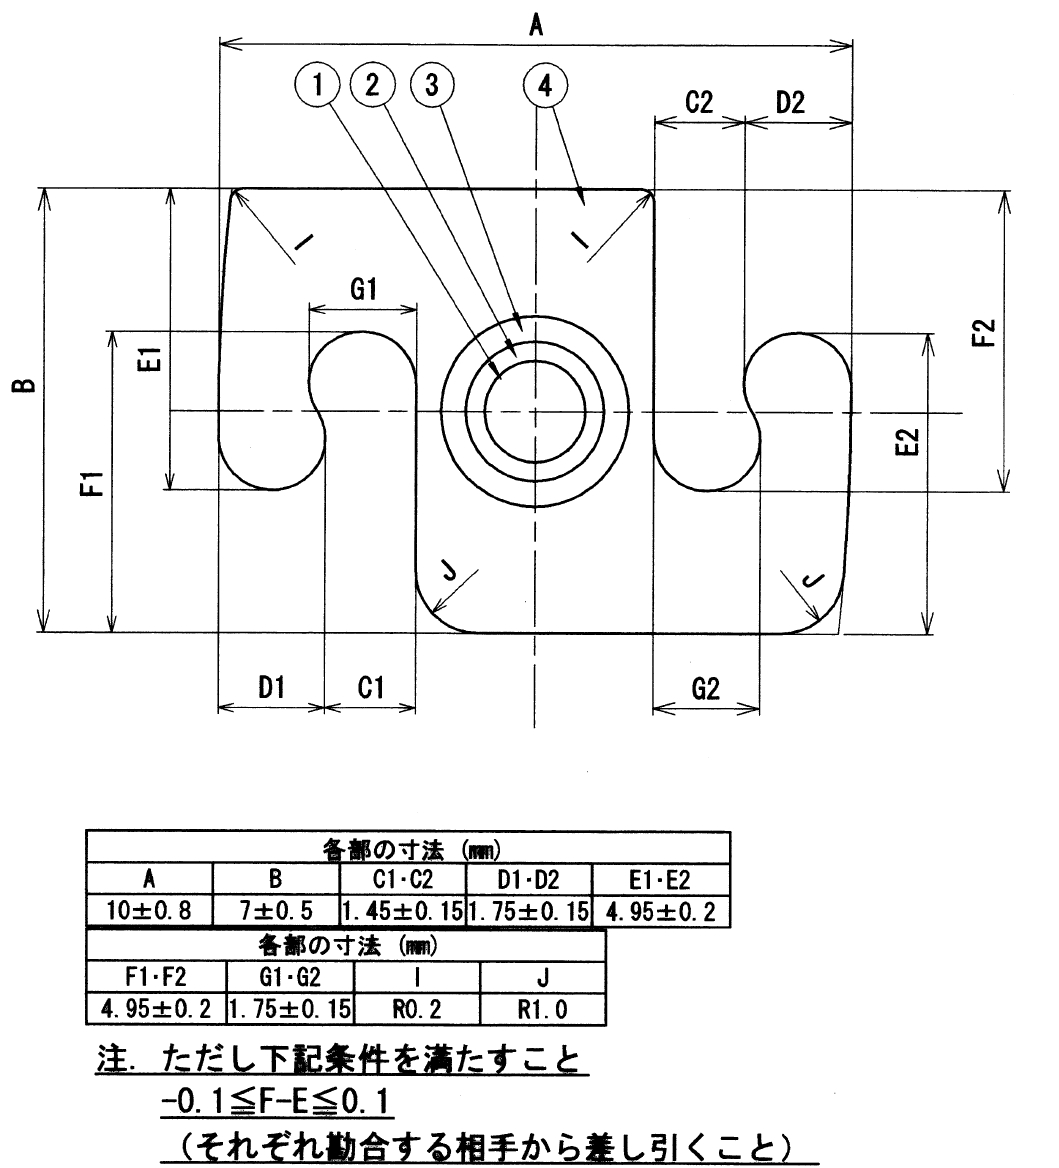
\includegraphics[width=\columnwidth]{SC_M-10-7.jpg}
    \caption{right}
    \label{fig:SC_M-10-7}
  \end{minipage}
\end{figure} 

この SC 用リボンケーブルは

\chapter{目的}
実験・シミュレーションの目的を簡潔に記す
\chapter{実験方法/解析方法}
実験・シミュレーションの内容を簡潔に記す
箇条書きもOK
\chapter{結果}
実験・シミュレーションの結果を簡潔に記す
箇条書きもOK
\chapter{考察 }
実験・シミュレーションの考察を簡潔に記す
箇条書きもOK
\chapter{結論}
結論を記す
目的と結論が一対になっているかを確認する
箇条書きもOK
\chapter{今後の進め方}
   今後の進め方を記す
   箇条書きもOK
\chapter{参考報告書・文献}
   関係する報告書・文献を記す


\end{document}